\documentclass{beamer}
\usepackage[utf8]{inputenc}
\usepackage[russian]{babel}
\usepackage{hyperref}
\usepackage{xcolor}
\usepackage{graphicx}

\begin{document}

\title[]{Критерий полноты для класса планарных предикатных схем}
\author{И.\,Ю.~Василевская}

\institute{
	{\em Научный руководитель}:\\к.ф.м.н. М.\,С.~Шуплецов \\
    \vspace{2.0cm}
}
\date{Москва, 2013}

\begin{frame}
	\maketitle
\end{frame}

\begin{frame}
	\frametitle{Обзор}

	\begin{block}{Задача синтеза}
		\begin{itemize}
			\item 30-40 годы прошлого века, Клод Шеннон
            \item для определенного класса дискретных управляющих систем
			\item структура схемы~-- граф специального вида
			\item функционирование схемы~-- реализуемая система булевых функций
		\end{itemize}
	\end{block}

	\begin{block}{Классы дискретных управляющих устройств}
		\begin{itemize}
			\item функциональные
			\item проводящие
			\item предикатные
		\end{itemize}
	\end{block}
\end{frame}

\begin{frame}
    \frametitle{Проектирование СБИС}

    \begin{block}{Основные этапы}
        \begin{itemize}
            \item Системное проектирование, C/C++, SystemC
            \item Аппаратное проектирование и верификация, Verilog/VHDL
            \item Физическое прототипирование, предварительное размещение элементов
            \item Проектирование и верификация топологии кристалл, трассировка, экстракция паразитных
            параметров
        \end{itemize}
    \end{block}

    \begin{block}{Трассировка}
        Ограничение на число пересечений контактов $\implies$ существенна минимизация числа реберных пересечений 
    \end{block}
\end{frame}

\begin{frame}{Описание модели}

    \begin{block}{Определение}
        \textit{Схема из предикатных элементов}~--- помеченный
         неориентированный двудольный граф:

        \begin{itemize}
            \item каждая вершина из первой доли помечена некоторым множеством символов из алфавита X и/или 
             множеством символов из алфавита Y. 
             Алфавит $X$ соответствует \textit{входным} переменным предиката, а $Y$~-- его внутренним переменным 

            \item каждая вершина второй доли помечена некоторым символом $\pi_i$ из множества $\Pi$ и 
            соединена $k$ ребрами, пронумерованными числами $1, \dots, k$, с вершинами из первой доли.
        \end{itemize}
    \end{block}
\end{frame}

\begin{frame}{Функционирование модели} 

    \begin{block}{Функционирование $\pi(x_1, \dots, x_n)$}
    \begin{itemize}
            \item Определяется допустимостью состояния схемы на наборе $\alpha$
            \item Задается его характеристической функцией $\chi_{\pi}$: 
                  $\Pi(x_1, \dots, x_n) = \{ \alpha | \chi_{\pi}(\alpha) = 1 \}$.
         \end{itemize}
    \end{block}

    \begin{block}{Оcновные операции}
        \begin{itemize}
            \item Суперпозиция с отождествлением полюсов
            \item Проекция по переменной
            \item Подстановка констант: $\pi_0(x_1)=\{ (0) \}$, $\pi_1(x_1)=\{ (1) \}$
            \item Отрицание переменной: $\pi_{\neg}(x_1, x_2)=\{ (01), (10) \}$.
        \end{itemize}
    \end{block}
\end{frame}

\begin{frame}{Полнота}
        \begin{block}{Определение}
        $f (x_1, \ldots, x_n)$ сохраняет предикат $\pi(x_1, \ldots, x_m)$ $\iff$ $\forall n$  
        $\alpha^i = (\alpha_1^i, \ldots, \alpha_n^i)$: 
        $( f(\alpha_1^1, \ldots, \alpha_1^n), \ldots, f(\alpha_m^1, \ldots, \alpha_m^n) )$~--- допустимый набор.
        \end{block}

    \begin{block}{Предполные классы}
        \begin{itemize}
            \item{$T_0$}~-- сохранение 0;
            \item{$T_1$}~-- сохранение 1;
            \item{S}~-- сохранение $\bar{x}$;
            \item{K}~-- сохранение всех конъюнкций;
            \item{D}~-- сохранение всех дизъюнкций;
            \item{SM}~-- сохранение всех монотонных самодвойственных ФАЛ;
            \item{SL}~-- сохранение всех монотонных линейных ФАЛ.
        \end{itemize}
    \end{block}
\end{frame}

\begin{frame}{Критерий полноты для предикатных схем}
    \begin{block}{}
    \label{Post}
    Система из $B$ предикатов является полной $\iff$
    она не лежит целиком ни в одном из 7 предполных классов: $T_0, T_1, SM, SL, S, K, D$. 
    \end{block}
\end{frame}

\begin{frame}{Планарность}
    \begin{block}{Определение}
        Планарная предикатная схема~--- схема, которую можно уложить на плоскости без реберных пересечений 
        так, чтобы входы лежали на внешней границе. 
    \end{block}

    \begin{block}{Операции планарной суперпозиции}
        \begin{itemize}
            \item Проекция по переменной
            \item Ограниченная суперпозиция по 2 переменным
            \item Отождествление входов
            \item Подстановка констант
            \item Отрицание переменной
        \end{itemize}
    \end{block}

    \begin{block}{}
    Существует планарная реализация $\pi_0, \pi_1, \pi_{\neg}$ в произвольном полном базисе $B_n \implies$ доступны
    все операции планарной суперпозиции.
    \end{block}
\end{frame}

\begin{frame}{Идеи доказательства}
    \begin{block}{Избавление от пересечений}
        \begin{figure}[htb]
        \centering
        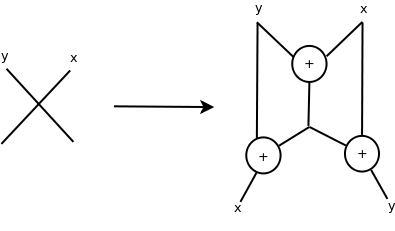
\includegraphics[width=0.5\textwidth]{intersection.png}
        \label{fig:xor}
        \end{figure}
    \end{block}
    \begin{block}{Лемма} 
    Существует планарная реализация $\pi_{linear} = \{(00), (01), (10), (11)\}$ в произвольном полном базисе $B_3$.
    \end{block}
    \begin{block}{Лемма} 
    Существует планарный переход от полного базиса $B_n$ к $B_{n-1}$.
    \end{block}
\end{frame}

\begin{frame}{Итоговые утверждения}
    \begin{block}{Теорема планаризации}
    \label{Theo2}
    Пусть дана непланарная предикатная схема $\Sigma$ в полном предикатном базисе $B$. 
    Тогда из $\Sigma$, применением операций планарной суперпозиции, можно получить схему $\Sigma'$,
    реализующую тот же предикат, что и $\Sigma$, но являющуюсь планарной.
    \end{block}
    \begin{block}{Критерий полноты для планарных предикатных схем}
    Система из $B$ предикатов является полной в классе планарных предикатных схем $\iff$
    она не лежит целиком ни в одном из 7 предполных классов: $T_0, T_1, SM, SL, S, K, D$. 
    \end{block}
\end{frame}

\begin{frame}
	\frametitle{Основные результаты}
    \begin{block}{}
	\begin{itemize}
        \item Определен класс операций планарной суперпозиции
		\item Сформулирован и доказан критерий полноты для планарных предикатных схем 
		\item Приведен алгоритм ``планаризации'', оценена его сложность
		\item Уточнена структура $\pi \notin SM$
	\end{itemize}
    \end{block}{}
\end{frame}

\begin{frame}{}
	\begin{center}
		\LARGE{Спасибо за внимание!}
	\end{center}
\end{frame}

\end{document}
